\usetheme{FINKI}
\usepackage{thumbpdf}
\usepackage{wasysym}
\usepackage{ucs}
\usepackage[T2A]{fontenc}
\usepackage[utf8]{inputenc}
\usepackage{pgf,pgfarrows,pgfnodes,pgfautomata,pgfheaps,pgfshade}
\usepackage{verbatim}
\usepackage{listings}
\usepackage{fancybox} 



\pdfinfo
{
  /Title       (AV5)
  /Creator     (Tomche Delev)
  /Author      (Tomche Delev)
}


\title[АВ5]{Аудиториски вежби 5}
\subtitle{Дијаграми на однесување\\Примери и вежби }
\author{Основи на софтверско инженерство}
\date{}
\pgfdeclareimage[width=0.6\paperwidth]{finki_logo}{finki_name}
\titlegraphic{\pgfuseimage{finki_logo}}



\begin{document}

\frame[plain]{\titlepage}

%Automatic table of contents
\section*{}
\begin{frame}
  \frametitle{Содржина}
  \tableofcontents[section=1,hidesubsections]
\end{frame}

\AtBeginSection[]
{
  \frame<handout:0>
  {
    \frametitle{Содржина}
    \tableofcontents[currentsection,hideallsubsections]
  }
}

\AtBeginSubsection[]
{
  \frame<handout:0>
  {
    \frametitle{Содржина}
    \tableofcontents[sectionstyle=show/hide,subsectionstyle=show/shaded/hide]
  }
}

\newcommand<>{\highlighton}[1]{%
  \alt#2{\structure{#1}}{{#1}}
}

\newcommand{\icon}[1]{\pgfimage[height=1em]{#1}}

\lstset{language=C,captionpos=b,
tabsize=4,frame=lines,
basicstyle=\scriptsize\ttfamily,
keywordstyle=\color{blue},
commentstyle=\color{lightgray},
stringstyle=\color{violet},
breaklines=true,showstringspaces=false}

%%%%%%%%%%%%%%%%%%%%%%%%%%%%%%%%%%%%%%%%%
%%%%%%%%%% Content starts here %%%%%%%%%%
%%%%%%%%%%%%%%%%%%%%%%%%%%%%%%%%%%%%%%%%%

\begin{frame}{Дијаграми на однесување}
\begin{itemize}
\item Дијаграм на кориснички случаи
\begin{itemize}
\item Ги опишува однесувањата на системот, целите на корисникот, надворешните
ентитети - актерите
\end{itemize}
\item Секвенцен дијаграм
    \begin{itemize}
    \item Се фокусира на временското подредување на пораките
    \end{itemize}
\item Колаборациски дијаграм
    \begin{itemize}
    \item Се фокусира на структурната организација на објектите и пораките
    \end{itemize}
\item Дијаграм на активности
    \begin{itemize}
        \item Го прикажува текот на контролата помеѓу активностите
    \end{itemize}
\end{itemize}
\end{frame}

\section{Дијаграм на кориснички случаи}

\begin{frame}[shrink=10]{Пример - подигање готовина од банкомат}{ATM}
\begin{block}{Цел}
Подигање на одреден износ на готовина од сметката на клиентот во банка
\end{block}
\begin{block}{Oпис}
Корисничкиот случај започнува кога клиентот ја вметнува кредитната картичка во банкоматот. 
Банкоматот го бара PIN кодот на корисникот. Системот го валидира PIN кодот. 
Доколку валидацијата е успешна, корисникот може да ја избере операцијата за подигање готовина, 
во спротивен случај се активира алтернативата 1 – се извршува неуспешна валидација. 
Клиентот го внесува износот на готовина кој сака да го подигне. 
Системот го проверува износот на сметката на клиентот и неговиот кредитен лимит. 
Доколку износот е во рамките на тековната состојба + кредитниот лимит, системот (банкоматот) 
ја издава готовината и ја печати потврдата, во спротивен случај алтернатива 2 – се извршува надминат износ.
\end{block}
\end{frame}

\begin{frame}[shrink=10]{Пример - подигање готовина од банкомат}
\begin{itemize}
  \item Aктери:
    \begin{itemize}
        \item Клиент
    \end{itemize}  
  \item Предуслов:
    \begin{itemize}
        \item Банкоматот мора да биде во состојба подготвен да прифати
        трансакција
        \item Банкоматот мора да има одредено количество готовина
        \item Банкоматот мора да има доволно хартија да отпечати потврда барем за една трансакција
    \end{itemize}  
  \item Пост - услов:
    \begin{itemize}
        \item Износот на готовина на сметката на клиентот добива вредност износ на сметката пред подигањето готовина минус подигнатиот износ
        \item Се печати потврда за подигнатиот износ
        \item Трансакцијата за подигање готовина се запишува во системската лог
        датотека
    \end{itemize}  
\end{itemize}  
\end{frame}

\begin{frame}{Пример - подигање готовина од банкомат}{Чекори при подигање на
готовина}
\begin{scriptsize}
\begin{tabular}{p{0.5\textwidth} | p{0.5\textwidth}}
\textbf{Акции на актерот} & \textbf{Акции на системот}\\
\hline
1. Започнува кога клиентот доаѓа до банкоматот & \\
\hline
2. Клиентот ја вметнува кредитната картичка во банкоматот & 3.Системот го
верификува идентитетот и статусот на клиентот \\
\hline
5. Клиентот избира операција  „Подигање готовина“ & 4. Системот прашува за тип
на операција \\
\hline
7. Клиентот го внесува износот на готовина & 6. Системот прашува за износ
наготовина за подигање\\
\hline
& 8. Системот проверува дали износот за подигање е дозволен\\
\hline
& 9. Системот ја издава готовината\\
\hline
& 10. Системот ја намалува состојбата на сметката за подигнатиот износ\\
\hline
& 11. Системот печати потврда\\
\hline
13. Клиентот ја подига готовината и потврдата & 12. Системот ја исфрла
кредитната картичка \\
\end{tabular}
\end{scriptsize}
\end{frame}


\begin{frame}{Пример - подигање готовина од банкомат}
\begin{itemize}
  \item Алтернативен тек на настаните:
  \begin{itemize}
    \item Чекор 3: Авторизацијата на клиентот е неуспешна. Се прикажува порака
за грешка, се откажува трансакцијата и се исфрла картичката.
  \item Чекор 8: Клиентот има недоволно висок износ на сметката. Се прикажува
  порака за грешка и се оди на чекор 6.
  \item Чекор 8: Клиентот го пречекорува дозволениот минус. Се прикажува порака
  за грешка и се оди на чекор 6.
\end{itemize}
  \item Исклучок како тек на настаните:
  \begin{itemize}
  \item Прекин на електричната енергија во процесот на трансакцијата пред чекор 9, откажување на трансакцијата и исфрлање на картичката
\end{itemize}
\end{itemize}
\end{frame}

\begin{frame}{Пример - подигање готовина од банкомат}
\begin{itemize}
  \item Првата метода за идентификација на корисничкиот случај е базирана на актерите:
  \begin{itemize}
    \item Се идентификуваат актерите кои се поврзани со системот или со организацијата.
  \item За секој актер, се идентификуваат процесите кои ги иницираат или во кои учествуваат.
\end{itemize}
  \item Втората метода за идентификација на корисничкиот случај е базирана на настаните:
  \begin{itemize}
  \item Се идентификуваат надворешните настани на кои системот мора да одговори.
  \item Настаните се ставаат во релација со актерите и со корисничките случаи.
\end{itemize}
\end{itemize}
\end{frame}

\begin{frame}{Пример - подигање готовина од банкомат}
Следните прашања можат да се користат за помош при идентификација на
корисничките случаи за еден систем:
\begin{itemize}
  \item Кои се задачите на секој актер?
  \item Дали кој било актер креира, запишува, менува, брише или чита информација
  во/од системот?
  \item Кои кориснички случаи ќе ја креираат, запишуваат, менуваат, бришат или
  читаат оваа информација?
  \item Дали некои актери ќе треба да го информираат системот за ненадејни
  надворешни промени?
  \item Дали кој било актер ќе треба да биде информиран за одредени појави во
  системот?
  \item Дали сите функционални барања можат да бидат претставени во корисничкиот
  случај?
\end{itemize}
\end{frame}
    
    
\begin{frame}{Пример - подигање готовина од банкомат}
\begin{center}
    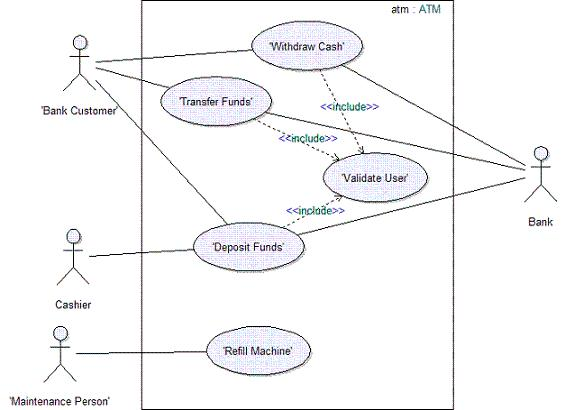
\includegraphics[scale=0.4]{images/atm_usecase.jpg}
\end{center}
\end{frame}

\section{Секвенцен дијаграм}

\begin{frame}{Пример - подигање готовина од банкомат}
\begin{itemize}
  \item Интеракциски дијаграм кој моделира едно сценарио кое се извршува во системот
\begin{itemize}
  \item Го моделира текот на контролата со временско подредување
  \item Го нагласува предавањето на пораки во однос на времето
  \item Покажува едноставна итерација и разгранување 
\end{itemize}
\item Моделот претставува сценарио за подигање готовина од банкомат од
претходниот кориснички случај. Клиентот може да подигне готовина од банкоматот. 
Системот користи стандардна процедура за валидација на кредитната картичка и PIN кодот на клиентот.
\end{itemize}
\end{frame}
    
\begin{frame}{Пример - подигање готовина од банкомат}
\begin{itemize}
  \item Главни објекти:
\begin{itemize}
  \item Клиент
  \item Банкомат
  \end{itemize}
  \item Опис на почетокот на главниот тек на настани во ова сценарио:
  \begin{itemize}
  \item Клиентот пристапува до банкоматот и ја вметнува кредитната картичка.
  \item Системот бара автентификација (PIN код).
\end{itemize}
  \item Преведете го текот во соодветен систем на настани (влез и одговор, input and response).
  \item Конструирајте секвенцен дијаграм базиран на овие информации.
\end{itemize}
\end{frame}

\begin{frame}{Пример - подигање готовина од банкомат}
\begin{enumerate}
  \item Клиентот пристапува до банкоматот и ја вметнува кредитната картичка.
  \item Системот бара од клиентот автентификација (PIN код).
  \item Клиентот го внесува PIN кодот.
  \item Системот му дозволува на клиентот да избере услуга.
  \item Клиентот избира подигање готовина.
  \item Системот прашува за износ на готовината.
  \item Клиентот го внесува износот.
  \item Системот прикажува дека трансакцијата е успешна, ја исфрла картичката и ја предава готовината.
  \item Клиентот ги зема картичката и готовината.
\end{enumerate}
\end{frame}

\begin{frame}{Пример - подигање готовина од банкомат}
\begin{center}
    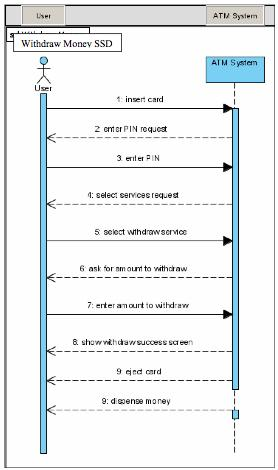
\includegraphics[scale=0.4]{images/sequence.jpg}
\end{center}
\end{frame}

\begin{frame}{Зошто се употребува секвенцен дијаграм}{Зошто не се програмира?}
\begin{itemize}
  \item Секвенцниот дијаграм е прилично блиску до нивото на изворен код на
  алгоритам.
  \item Зошто едноставно не се кодира алгоритмот веднаш, туку се црта секвенцен
  дијаграм?
  \begin{itemize}
  \item Добар секвенцен дијаграм е барем малку над нивото на реалниот код (не секоја линија код се црта на дијаграмот)
  \item Секвенцните дијаграми се независни од програмскиот јазик и може да се
  имплементираат во различни јазици
  \item Тие што не знаат да програмираат можат да работат секвенцни дијаграми
  \item Поедноставно е тимски да се направи секвенцен дијаграм
  \item Може да се видат повеќе објекти и класи истовремено на иста страна (визуелен опсег)
\end{itemize}
\end{itemize}
\end{frame}

\section{Колаборациски дијаграм}

\begin{frame}{Колаборациски дијаграм}
\begin{itemize}
  \item Ја нагласува организацијата на објектите кои учествуваат во интеракцијата
  \item Класифицира улоги
  \item Асоцијација
  \item Пораки, тек и секвенцирање
  \item Ја опишува интеракцијата помеѓу класите и асоцијациите
  \item Се моделира како размена на пораки помеѓу класите и нивните асоцијации
  \item Еден вид на интеграциски дијаграми
\end{itemize}
\end{frame}

\begin{frame}{Колаборациски дијаграм}
\begin{itemize}
  \item Класни улоги
\begin{itemize}
  \item Кои претставуваат улоги кои објектите може да ги играат за време на интеракцијата
\end{itemize}
  \item Асоцијациски улоги
\begin{itemize}
  \item Кои претставуваат улоги кои врските може да ги играат со интеракцијата
\end{itemize}
  \item Текови на пораки
\begin{itemize}
  \item Кои претставуваат пораки кои се испратени помеѓу објектите преку линкови
  \item Линковите ја вршат размената на пораката
\end{itemize}
\end{itemize}
\end{frame}

\begin{frame}{Пример - подигање готовина од банкомат}
\begin{center}
    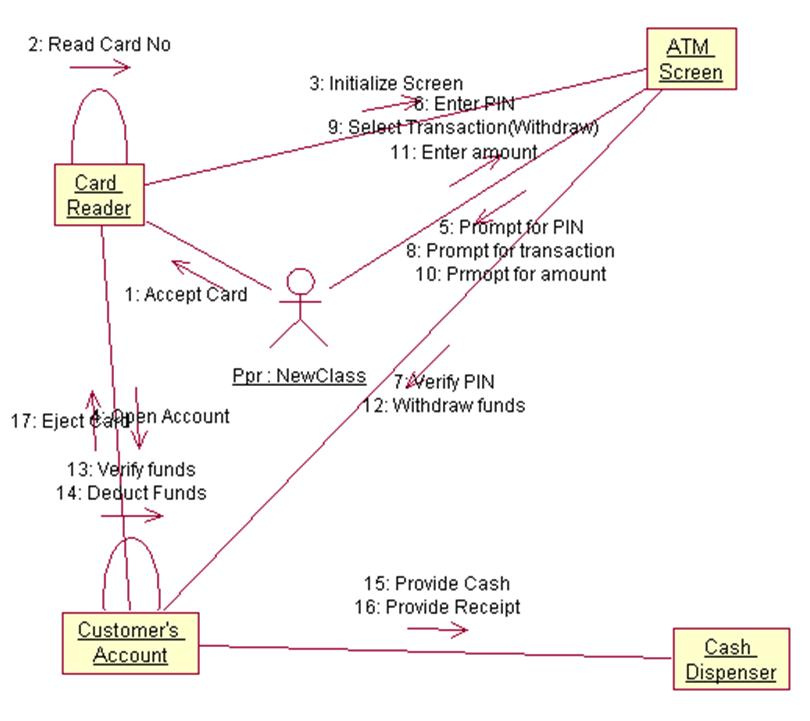
\includegraphics[scale=0.2]{images/colaboration.jpg}
\end{center}
\end{frame}

\section{Дијаграм на активности}

\begin{frame}{Дијаграм на активности}
\begin{itemize}
  \item Моделира контрола и информациски тек на процедура или процес
  \item Корисно е ако контролата е главно синхрона
  \item Состојба на акција
\begin{itemize}
  \item Состојба во која се извршува некој процес
  \item Активност, задача
  \item Состојбата завршува кога завршува процесот
  \item После завршување, состојбата на акција може да доведе до друга состојба на акција
  \item Се користат специјални симболи за почеток и крај на процес
\end{itemize}
\end{itemize}
\end{frame}

\begin{frame}{Пример - подигање готовина од банкомат}
\begin{center}
    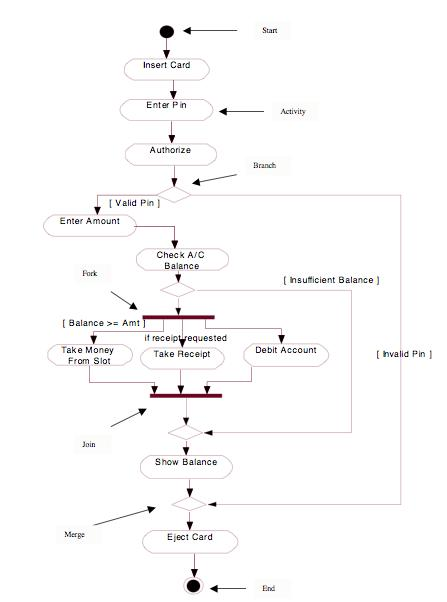
\includegraphics[scale=0.35]{images/activity.jpg}
\end{center}
\end{frame}

\begin{frame}{Материјали}{}
	Предавања, аудиториски вежби, соопштенија\\
	\href{http://courses.finki.ukim.mk/}{\textbf{courses.finki.ukim.mk}}
	\vfill
	{\Huge Прашања ?}
\end{frame}

\end{document}
